\subsubsection{Configuring and Resetting MFA}

\newline
Multi-Factor Authentication (MFA) is required to access OpenScienceLab resources.

Currently, we support TOTP-based authentication, with plans to add hardware
key (ex. Yubikey) authentication in future updates.

\begin{itemize}
\item Watch:~Log~In~and~Set~Up~MFA
\item Before~You~Begin
\item Setup~Steps
\item Resetting~MFA
\item Troubleshooting
\end{itemize}


\bigskip
\centerline{\rule{13cm}{0.4pt}}
\bigskip

\paragraph{Watch: Log In and Set Up MFA}\label{Watch-Log-In-and-Set-Up-MFA}


\bigskip
\centerline{\rule{13cm}{0.4pt}}
\bigskip

\paragraph{Before You Begin}\label{Before-You-Begin}

A TOTP-enabled MFA application is required to use OpenScienceLab resources.
While the most widely utilized approach is through a smartphone application,
there are also several desktop clients that provide this functionality.

\begin{framed}
\textbf{MFA App Support}\\
\bigskip\noindent
\begin{tabular}{p{\dimexpr 0.250\linewidth-2\tabcolsep}p{\dimexpr 0.250\linewidth-2\tabcolsep}p{\dimexpr 0.250\linewidth-2\tabcolsep}p{\dimexpr 0.250\linewidth-2\tabcolsep}}
\toprule
Application & Desktop Support & Android Support & iOS Support \\
\hline
KeePassXc & ✅ & ❌ & ❌ \\
Enpass & ✅ & ✅ & ✅ \\
Cisco Duo & ✅ & ✅ & ✅ \\
\href{http://Authenticator.cc}{Authenticator.cc}* & ✅ & ✅ & ✅ \\
Bitwarden** & ✅ & ✅ & ✅ \\
FreeOTP & ❌ & ✅ & ✅ \\
Google Authenticator & ❌ & ✅ & ✅ \\
Microsoft Authenticator & ❌ & ✅ & ✅ \\
Aegis Authenticator & ❌ & ✅ & ❌ \\
\bottomrule
\end{tabular}

\bigskip* Browser based

** TOTP supported in paid version only
\end{framed}


\bigskip
\centerline{\rule{13cm}{0.4pt}}
\bigskip

\paragraph{Setup Steps}\label{Setup-Steps}

\begin{enumerate}
\item Log into OpenScienceLab normally. Leave the ``MFA'' field on the login page blank.
\item Click ``Configure New MFA Device'' in the Navigation Bar at
the top of the page.
\item Configure your MFA device:\begin{enumerate}
\item If using a smartphone application, scan the QR code using the
application's ``Scan QR Code'' feature.
\item If using a desktop application, copy the OTP Secret into the ``TOTP'' field
\end{enumerate}


\item Enter the current 6-digit MFA code generated by your application into the ``Code 1'' field
on the ``Configure New MFA Device'' page.
\item When the code changes, enter the new code into the ``Code 2'' field on the same
page and click the ``Check MFA Codes'' button.
\item If the check is successfull, navigate back to the home page by clicking ``Home''
in the Navigation Bar at the top of the page and continue using OpenScienceLab
as normal.
\end{enumerate}


\bigskip
\centerline{\rule{13cm}{0.4pt}}
\bigskip

\paragraph{Resetting MFA}\label{Resetting-MFA}

On occasion, you may wish or need to reconfigure MFA for your OSL account.

\begin{enumerate}
\item Navigate to \href{https://opensciencelab.asf.alaska.edu/}{opensciencelab}.


\item
\end{enumerate}

\begin{figure}[!htbp]
\centering
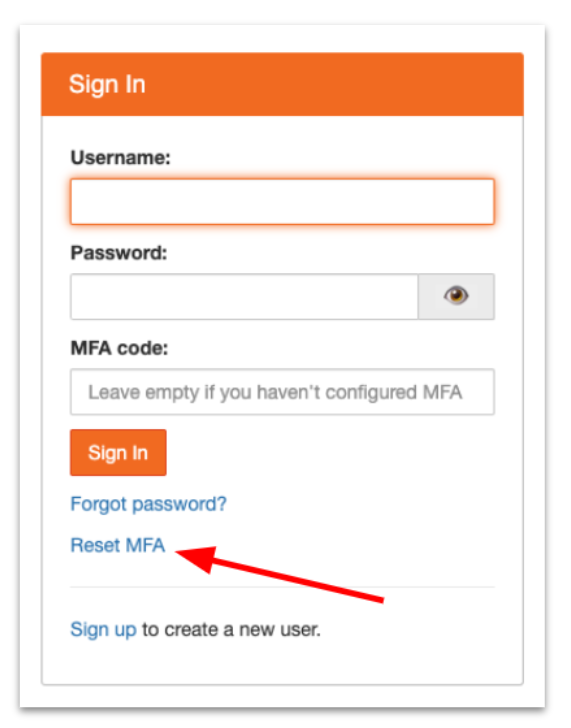
\includegraphics[width=0.4375\linewidth]{files/reset_mfa-236175c67c558a74caf5dfff2036ca1a.png}
\caption*{Click the "Reset MFA" link on the sign in card}
\end{figure}

\begin{enumerate}[resume]
\item
\end{enumerate}

\begin{figure}[!htbp]
\centering
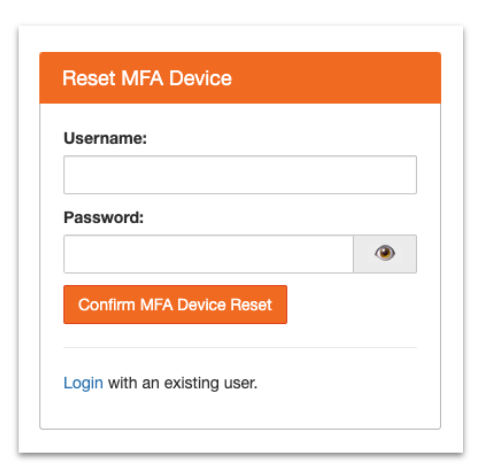
\includegraphics[width=0.4375\linewidth]{files/mfa_reset_form-ca56fa832e366f636d3f2771f45e7255.png}
\caption*{Complete the MFA reset form.}
\end{figure}

\begin{enumerate}[resume]
\item
\end{enumerate}

\begin{figure}[!htbp]
\centering
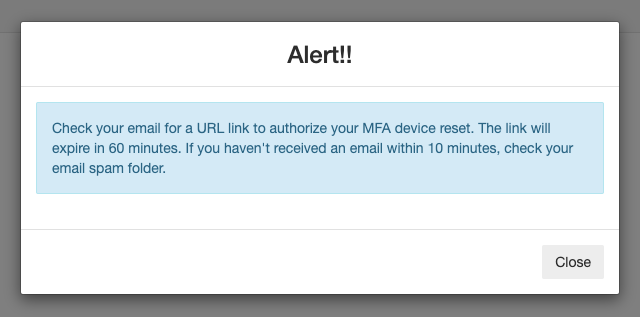
\includegraphics[width=0.625\linewidth]{files/mfa_update_alert-3e0a0f153977a430edaea4ff25e7887d.png}
\caption*{An alert will appear directing you to click an emailed verification link within 60 minutes.}
\end{figure}

\begin{enumerate}[resume]
\item
\end{enumerate}

\begin{figure}[!htbp]
\centering
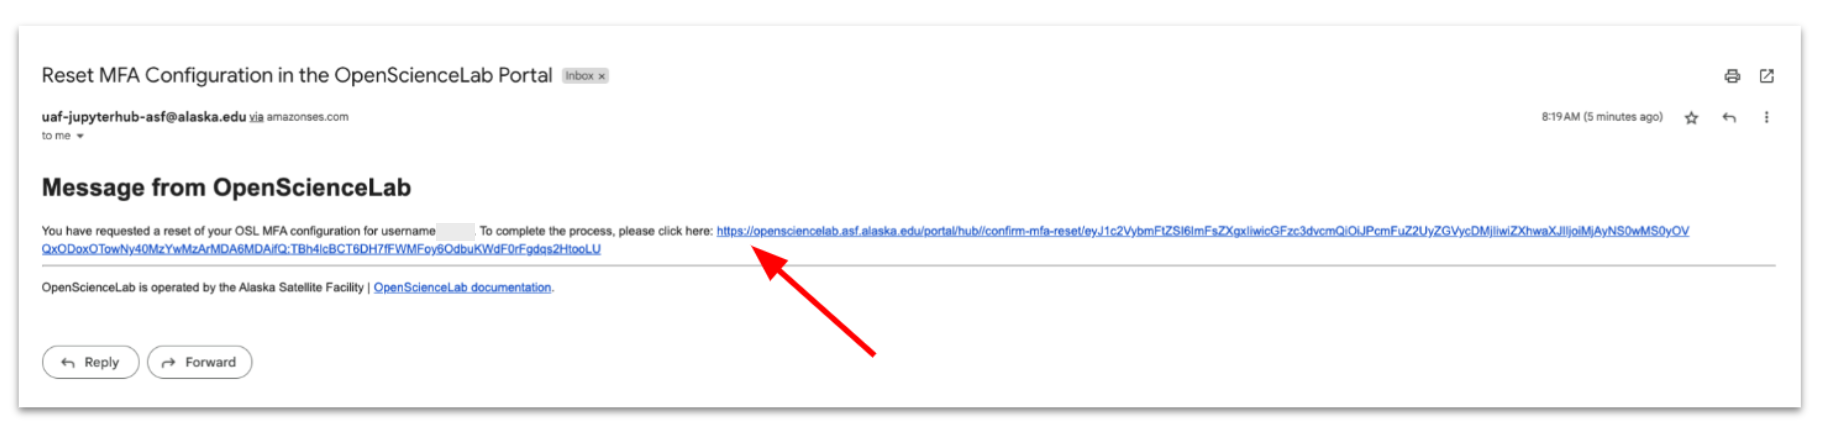
\includegraphics[width=0.7\linewidth]{files/mfa_reset_email-c0d983a161cc3d91309ff3be25196636.png}
\caption*{Click the verification link in the email.}
\end{figure}

\begin{enumerate}[resume]
\item Sign into OpenScienceLab, leaving the MFA field empty.
\item \textbf{Follow the Setup Steps above to setup a new MFA device.} You will not be able to access any labs until you setup a new MFA device.
\end{enumerate}


\bigskip
\centerline{\rule{13cm}{0.4pt}}
\bigskip

\paragraph{Troubleshooting}\label{Troubleshooting}

\begin{enumerate}
\item If the MFA Code check is not successful, there are two potential issues:\begin{enumerate}
\item One of the codes was mis-typed.
\item The secret was not properly put into the MFA application.
\end{enumerate}


\item Test again with another two \textit{consecutive} codes, and if the verification step fails
again, check that the OTP Secret on the page matches the secret in your application.
\item If all else fails, refresh the page. This will generate a new code, which you
can then use to follow the same steps above.
\end{enumerate}

For additional issues and further troubleshooting, please email
\href{mailto:uso@asf.alaska.edu}{uso@asf.alaska.edu}